%*****************************************
\chapter{Der Graphen Generator}\label{ch:generierung}
%*****************************************
Da wir die Theorie hinter sozialen Netzwerken und der Analyse dieser erarbeitet haben, wollen wir uns nun damit beschäftigen, wie wir typische soziale Netzwerke generieren können. 
Zunächst bietet es sich oftmals an, da Facebook und Instagram der Informationspflicht unterliegen, die eigenen social Media Daten anzufordern. Meist spiegelt dieser Datensatz gelikete und kommentierte Posts der Nutzer*innen wieder, oder verfasste Nachrichten und gesuchte Inhalte.
Bei den ersten Visualisierungsversuchen wird bereits klar, dass diese Daten für eine wissenschaftliche Arbeit nicht brauchbar sind, da es sich bei den erstellten Plots und Ergebnissen nicht um \textit{ typische soziale Netzwerke} handelt. Vielmehr bestehen diese meist aus einem Kernknoten, also einem sogenannten sternförmigen Graphen. Aber auch die Abbildung \ref{fig:OwnData} ist typisch für die Visualisierung der eigenen Daten. Diese besteht aus unzähligen einzelnen Teilgraphen, welche lediglich eine weitere Verbindung aufweisen. Auch finden wir keine Cliquen oder Bridgen (Brücken) in solchen Graphen, was ebenfalls dafür spricht, dass es sich um kein \textit{typisches soziales Netzwerk} handelt. \\
\FloatBarrier
\begin{figure}[h!]
    \centering
    %\hspace*{-1cm}
    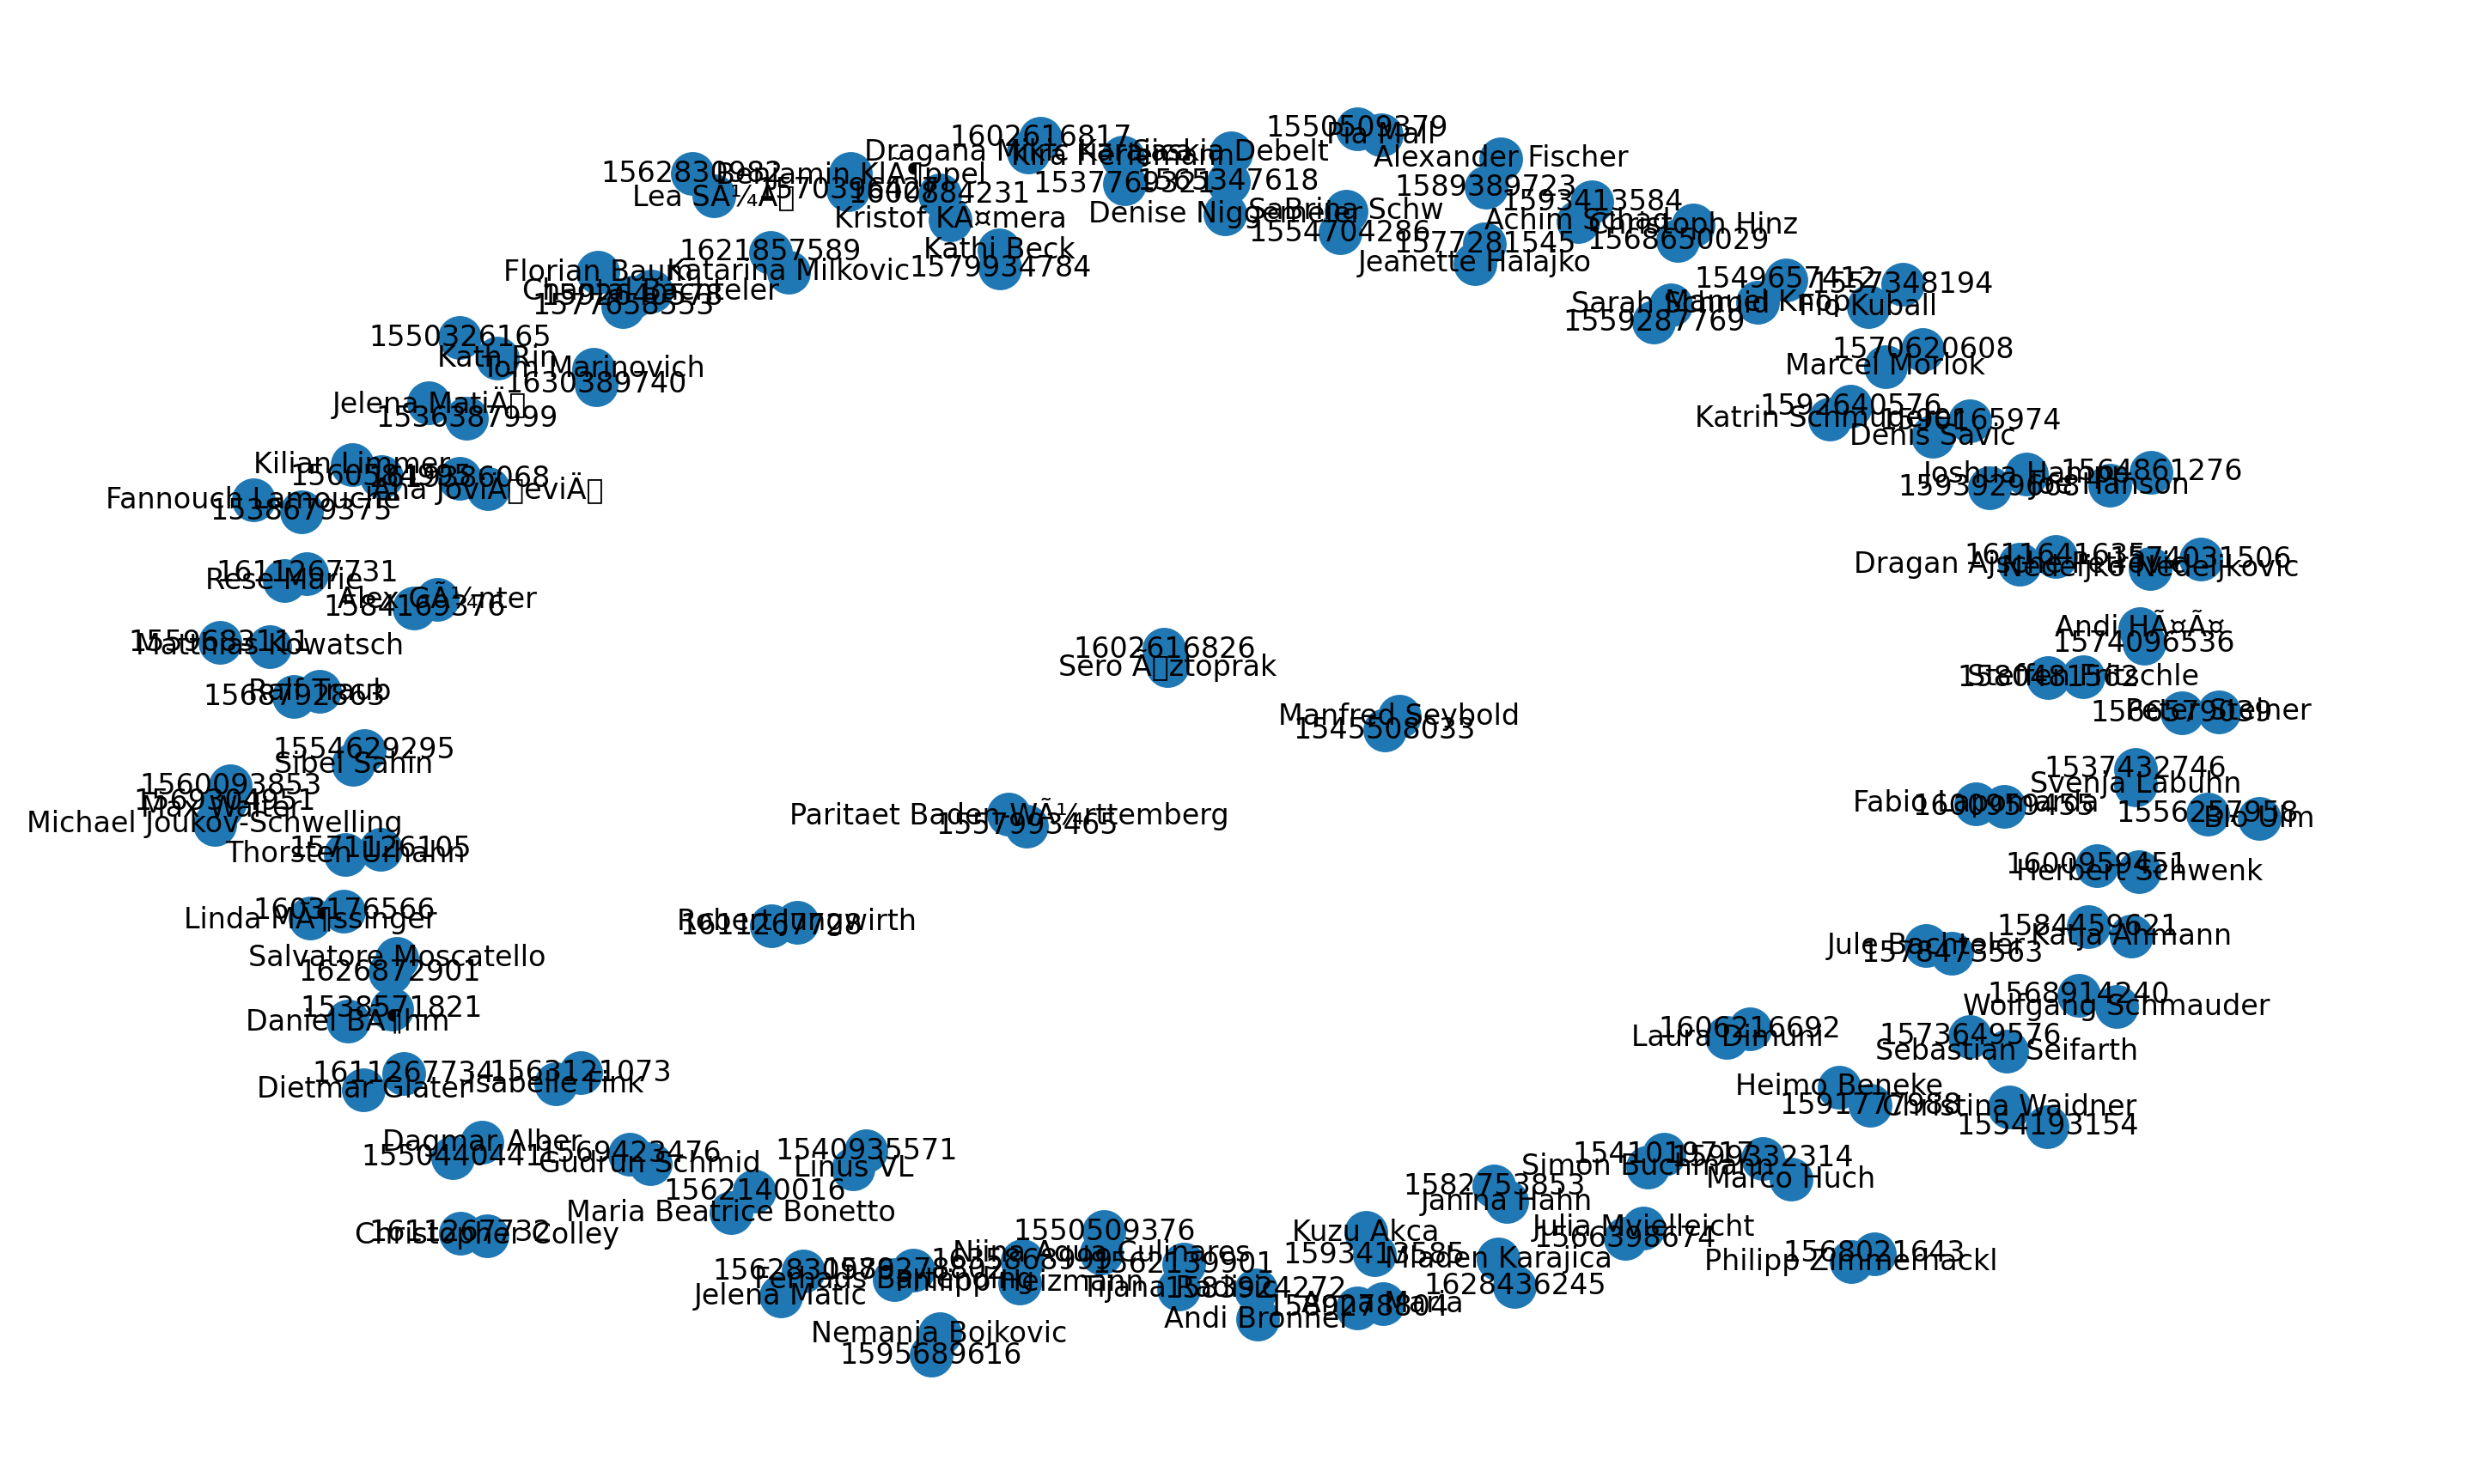
\includegraphics[width=0.7\textwidth]{Graphics/PlotOwnData.png}
    \caption{Erste Versuche eines Sozialen Netzwerks, \\
    selbst erstellt}
    \label{fig:OwnData}
\end{figure}
\FloatBarrier

Eine weitere Schwierigkeit ist bei diesen Graphen die Interpretation der Kanten, denn diese sind teilweise nicht eindeutig. 
Facebook gibt lediglich bestimmte IDs bekannt, doch welche exakte Bedeutung diese haben bleibt unklar.

\section{Generierung eines random Netzwerk-Plots mit vordefinierten Modellen} 
Bei einer endlichen Anzahl von Knoten \textit{n} gibt es auch eine endliche Anzahl von Graphen, die aus diesen Knoten erzeugt werden können. Hierbei wächst die Anzahl der Graphen mit \textit{n} Knoten exponentiell.
Ein Zufallsgraph ist nur einer dieser Graphen, der durch einen Zufallsprozess erzeugt werden kann.
Wenn von \textit{Zufallsgraphen} die Rede ist, wird in den meisten Fällen das \textit{Erdős-Rényi-Modell} als Graphengenerator verwendet (benannt nach den Mathematikern Paul Erdős und Alfréd Rényi). Eine wichtige Eigenschaft von, auf diese Weise erzeugten Zufallsgraphen ist, dass alle Konstellationsmöglichkeiten des Graphen gleichverteilt erzeugt werden \cite{Generators}.
Neben dem Erdős-Rényi-Modell, gibt es noch viele weitere Methoden zur random Netzwerkmodellierung \cite{Generators}.
\begin{itemize}
    \item die $"$ dense$\_$gnm$\_$random$\_$graph$"$ liefert einen $G_{n,m}$-Zufallsgraphen.
    Bei dem $G_{n,m}$-Modell wird ein Graph gleichmäßig zufällig aus der Menge aller Graphen mit $n$ Knoten und $m$ Kanten ausgewählt.
    \item bei der $"$Newman–Watts–Strogatz small-world graph$"$-Modellierung wird zunächst ein Ring mit $n$ Knoten erzeugt. Dann wird jeder Knoten im Ring mit seinen $k$ nächsten Nachbarn verbunden (oder $k - 1$ Nachbarn, wenn $k$ ungerade ist). Anschließend wird für jede Kante $(u, v)$ im zugrundeliegenden $"$ $n$-Ring mit $k$ nächsten Nachbarn$"$, mit der Wahrscheinlichkeit $p$, eine neue Kante $(u, w)$ mit einem zufällig ausgewählten bestehenden Knoten w hinzugefügt. Im Gegensatz zu $"$watts$\_$strogatz$\_$graph()$"$ werden bei dieser Methode keine Kanten entfernt
    \item Die $"$random$\_$regular$\_$graph $"$-Modellierung gibt einen zufälligen $d$-regulären Graphen mit $n$ Knoten zurück.
    Der resultierende Graph hat keine Selbstschleifen oder parallele Kanten
    \item Die $"$barabasi$\_$albert$\_$graph$"$-Modellierung hingegen liefert einen Zufallsgraphen nach dem Barabási-Albert-Präferenzmodell.
    Ein Graph mit $n$ Knoten wird durch Anhängen neuer Knoten mit jeweils $m$ Kanten erzeugt, die bevorzugt an bestehende Knoten mit hohem Grad angehängt werden.
    \item Die $"$powerlaw$\_$cluster$\_$graph$"$-Modellierung ist im wesentlichen das Barabási-Albert (BA)-Wachstumsmodell mit dem zusätzlichen Schritt, dass für jede zufällige Kante die Chance besteht, dass ebenfalls eine Kante zu einem seiner Nachbarn besteht (und damit ein Dreieck entsteht) \cite{Generators}.
\end{itemize}

\FloatBarrier
\begin{figure}[h!]
    \centering
    \hspace*{-1.5cm}
    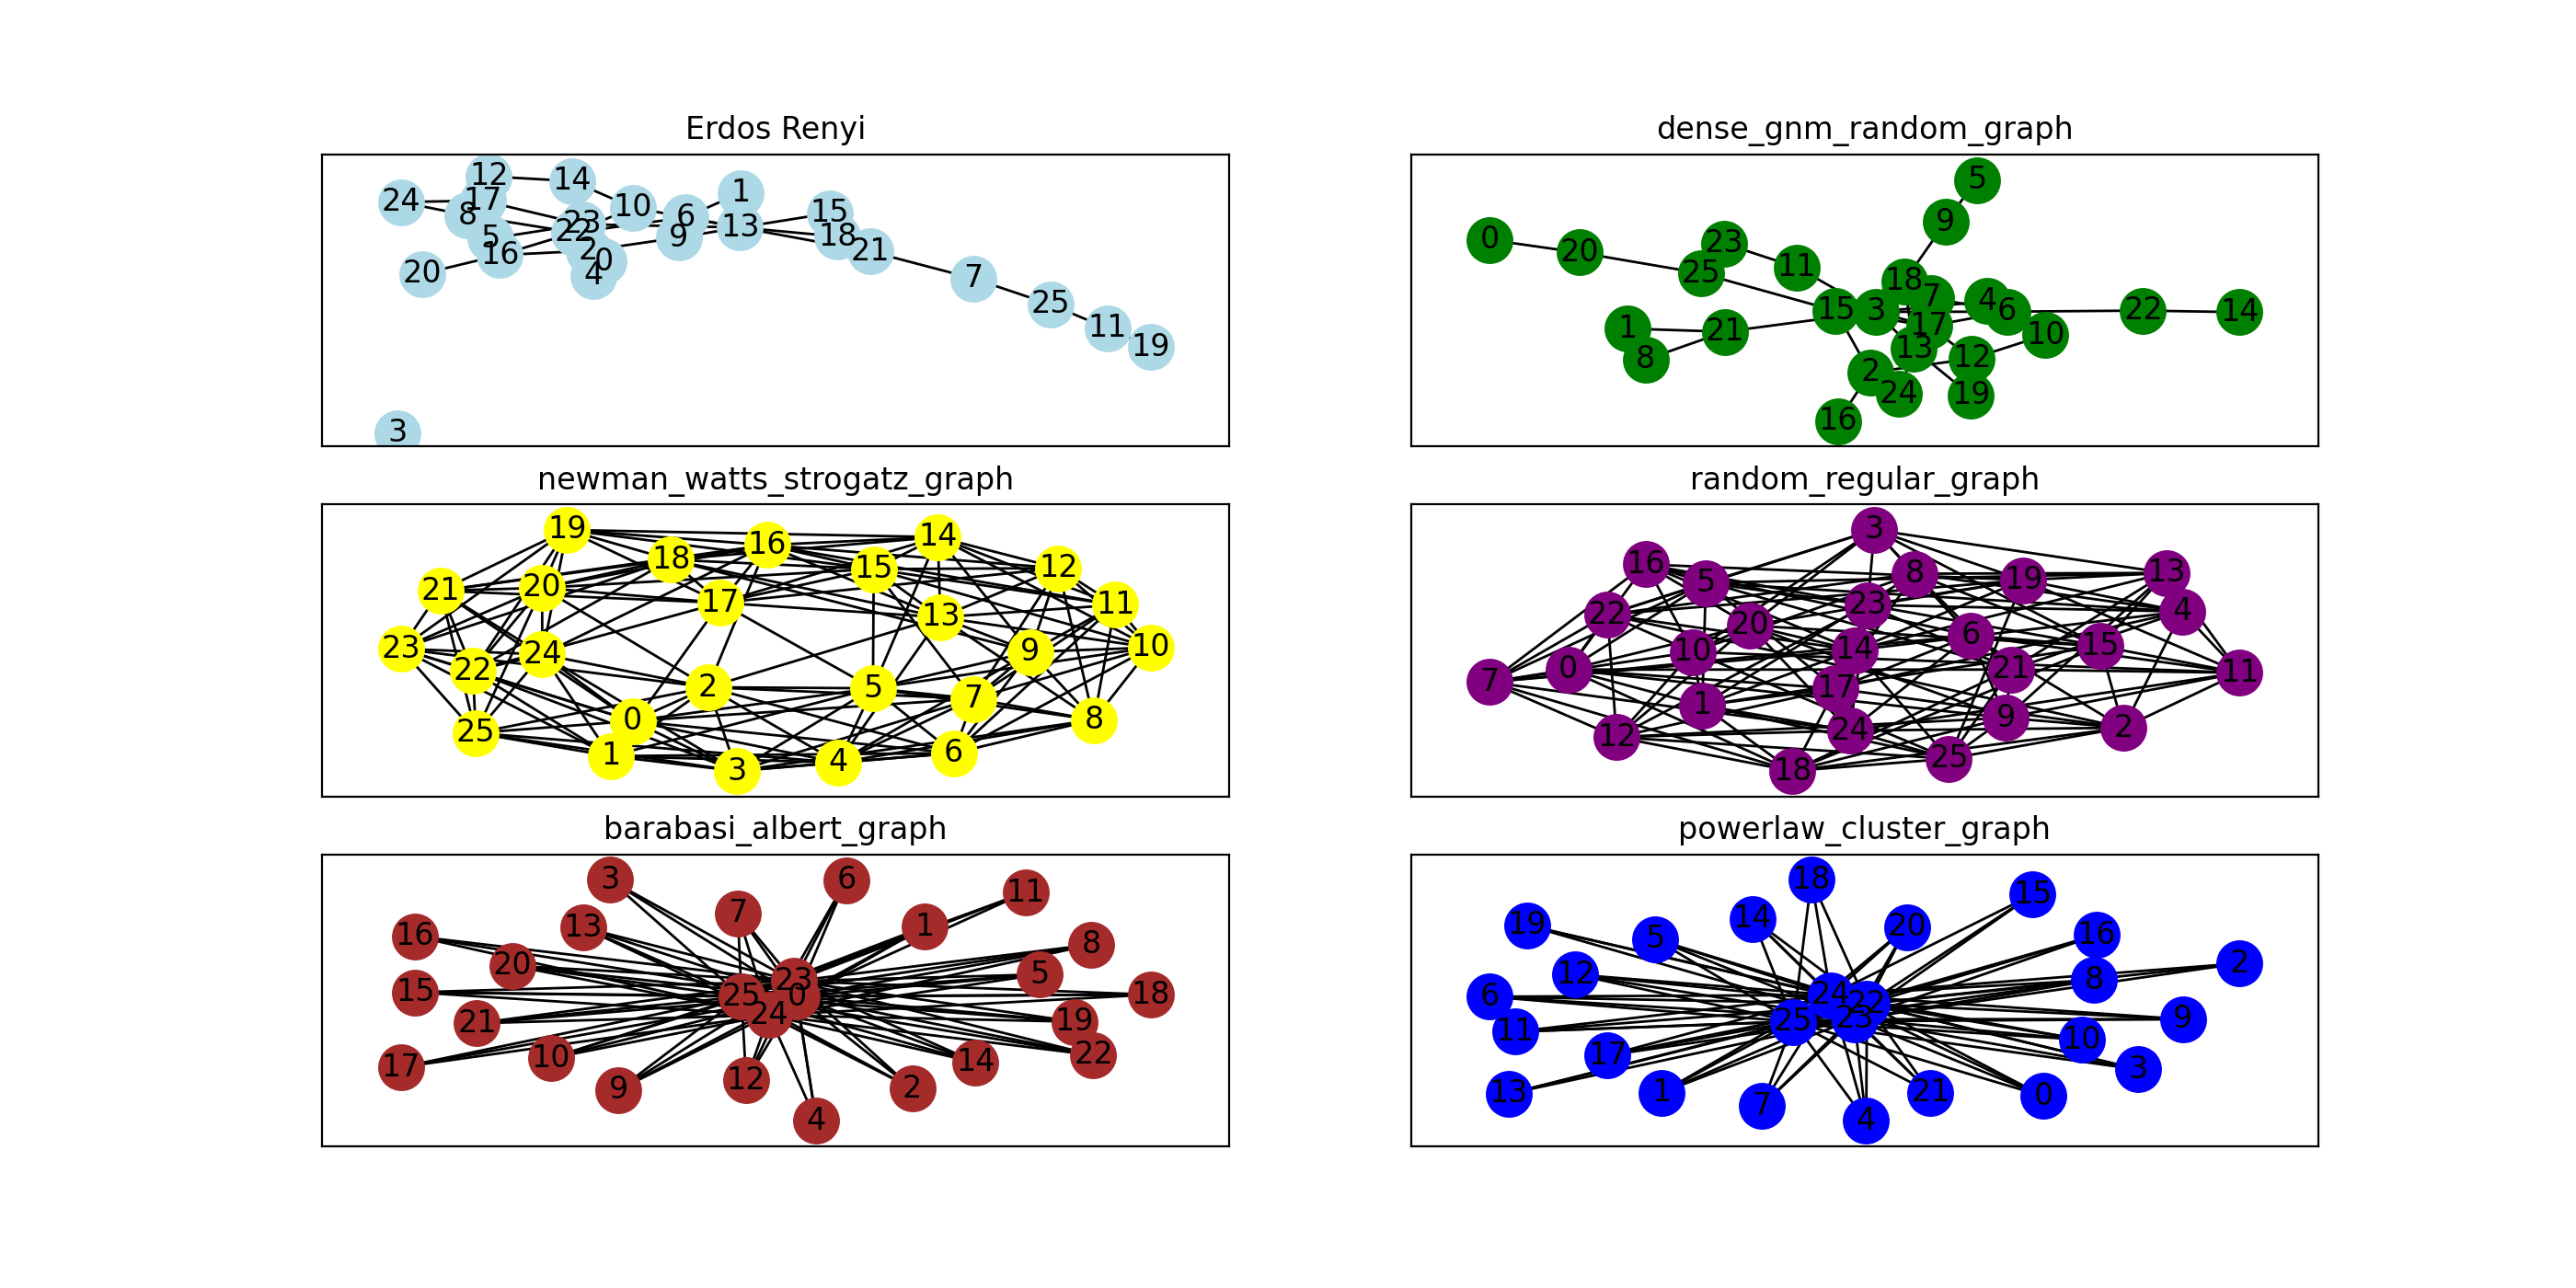
\includegraphics[width=1.2\textwidth]{Graphics/6Random.png}
    \caption{zufällig erstellte Graphen mit 25 Knoten nach den jeweiligen Methoden}
    \label{RandomGraphen}
\end{figure}
\newpage

Bei den Graphen \ref{RandomGraphen} wurde lediglich eine visuelle Interpretation durchgeführt und nicht den Graphen mit den jeweiligen Zentralitäten analysiert. Auf den ersten Blick erkennen wir, dass bei allen sechs Modellen Unstimmigkeiten zu \textit{sozialen Netzwerken} auftreten. Beispielsweise bei dem \textit{Barabasi Albert Graph} unten links und dem \textit{Powerlaw cluster graph} unten rechts erkennen wir einzelne zentrale Knoten. Diese zentrale Knoten befinden sich in der Mitte des Plots und sind von vielen weiteren Knoten umgeben, die alle wiederum mit diesen zentralen Knoten verbunden sind. Auch der \textit{newman watts strogatz graph} und der \textit{random regular graph} entsprechen nicht den erwünschten \textit{sozialen Netzwerken}. Beide mittigen Plots sind ringförmig angeordnet und es scheint, als sei jeder Knoten mit jedem weiteren Knoten verbunden, was eine untypische Eigenschaft ist. Nun bleiben noch die beiden oberen Plots des \textit{Erdos Renyi-Graphen} und \textit{dense gnm random graph}, welche ebenfalls nicht unseren Erwartungen entsprechen. Der Plot des \textit{dense gnm radom graph} weist zwar einzelne Äste auf, die aus der Mitte des Plots verlaufen, doch haben wir generell wenige Cliquen und müssen feststellen, dass der Plot keine Cluster aufweist, weshalb dieses Modell ebenfalls nicht brauchbar ist. Bei dem \textit{Erdos Renyi Modell} haben wir die gleiche Problematik wobei hier noch das Problem hinzu kommt, dass wir einen isolierten Knoten finden. Ein isolierter Knoten ist im Zusammenhang mit Socialen Netwerken, ein Knoten der keinen Nachbarn besitzt, also Grad $0$ aufweist.
Dies würde beispielsweise auf Sozial Media, bezogen bedeuten, dass Nutzer*innen auf dieser Plattform angemeldet sind, die keinerlei Verbindungen besitzen. Dies kann durchaus der Fall sein, es ist aber sehr unwahrscheinlich, dass Menschen auf solchen Plattformen angemeldet sind und keinerlei Freunde haben oder andere Nutzer*innen. Deshalb muss auch bei diesem Modell kritisch hinterfragt werden, ob es sich bei den Graphen um ein \textit{soziales Netzwerke} handelt. Im Allgemeinen liegt die Vermutung liegt nahe, dass es bei den Netzwerken in \ref{RandomGraphen} zu Unstimmigkeiten mit unseren Erwartungen kommt, da wir lediglich \textbf{25} Knoten betrachten. Dies ist für ein \textit{soziales Netzwerk} durchaus zu wenig. Deshalb liegt nahe, dass wir Anpassungen durchführen müssen.

\section{Random Graphen Generierung}
Eine mögliche Optimierung erzielen wir, indem wir von den Random Graphen-Methoden, die wir im vorherigen Abschnitt kennegelernt haben, abweichen. Eine weitere Überlegung, um eine Optimierung zu erzielen ist, alle Formeln selbständig zu implementieren und nicht die bereits vordefinierten Funktionen zu verwenden. Zum einen sind diese vordefinierten Funktionen intransparent und daher auch fehleranfälliger, aber auch der Zugriff auf diese ist nicht ganz einfach. Zudem erlangen wir durch die eigenständige Implementierung der Zentralitäten ein noch besseres Verständnis für die Formeln dieser.
Für die Generierung eines \textit{sozialen Netzwerks} benötigen wir unter anderem eine Methode, die einzelne zufällige Graphen erstellt. 

\begin{algorithm}
\caption{Random Adjazenzmatrix}\label{randomAdjacency}
\begin{algorithmic}[1]
\Procedure{random adjacency matrix}{}
\State $\textit{matrix} \gets \text{zufällige Matrix der Größe (n,n) zufällig befüllt mit Werten zwischen 0 und 1}$
\For {\textit{i} liegt in der Matrix}
\State \textit{befülle die Diagonale der Matrix mit 1}.
\EndFor
\For {\textit{i und k} liegen in der Matrix}
\State \textit{setze die Wahrscheinlichkeit auf einen zufälligen Wert zwischen 0 und 1}.
\If{Matrix an der Stelle [i][k] größer als die Wahrscheinlichkeit ist}
\State \textit{setze die Matrix an dieser Stelle auf 0}
\Else 
\State \textit{setze diese Stelle auf 1}
\EndIf
\EndFor
\For {\textit{i} liegt in der Matrix}
\State \textit{was für Matrix an der Stelle [i][j] gilt, muss auch für [j][i] gelten}.
\State \textbf{RETURN} Matrix
\EndFor
\EndProcedure
\end{algorithmic}
\end{algorithm}

Dieser Algorithmus erstellt uns zufällige Matrizen, die aber erst noch zu einer großen Matrix zusammengefügt werden müssen. Hierfür benötigen wir eine Methode, wie den \textit{Graph appender}. Der Algorithmus dieser Methode soll wie folgt aussehen. 

\begin{algorithm}
\caption{alle Subgraphen zu einer Liste zusammenführen}\label{GraphAppender}
\begin{algorithmic}[1]
\Procedure{graph appender}{}
\State $\textit{graphs} \gets \text{leeres Array}$
\For {\textit{i} zwischen 1 und der Anzahl an Subgraphen / Matrizen}
\State $\textit{k} \gets \text{zufälliger integer, der die Größe des Subgraphen definiert}$
\State $\textit{p} \gets \text{zufälliger double zwischen 0 und 1 für die Wahrscheinlichkeit}$
\State \textbf{goTo} \text{Algorithm 1 mit den übergebenen Werten \textit{k und p}}
\State \text{füge random Matrix in graphs ein und } \textbf{RETURN} graphs 
\EndFor
\EndProcedure
\end{algorithmic}
\end{algorithm}

\newpage
Wir fügen also die einzelne Matrizen der Liste hinten an.
Nachdem wir nun eine Liste mit vielen zufällig erzeugten Matrizen generieren konnten, fehlt uns lediglich eine Methode, um die Graphen zusammenzuführen und sicherzustellen, dass die Teilgraphen miteinander verbunden sind. Der Algorithmus sieht hierfür wie folgt aus:

\begin{algorithm}
\caption{Graphs zusammenführen}\label{uniteGraphs}
\begin{algorithmic}[1]
\Procedure{unite graphs}{}
\If {\text{länge der Liste \textit{graphs} aus nur einem Element besteht}}
\State \text{gebe \textit{graphs} zurück}.
\EndIf
\State $\textit{dimesion} \gets \text{0}$
\State $\textit{big graph} \gets \text{Graph mit Nullen befüllt}$
\For{\textit{i} zwischen \textit{0 und der Länge von graphs}}
\State $\textit{Variable a} \gets \text{zufälliger integer zwischen 0 und Länge von graphs}$
\State $\textit{Variable b} \gets \text{zufälliger integer zwischen 0 und Länge von graphs}$
\For{\textit{j und k} zwischen \textit{0 und graphs}}
\State $\textit{l} \gets \text{summierte Länge von Graphs bis zur Stelle i}$
\State $\text{\textit{big graph} an der Stelle [(l+j)][(l+k)]} \gets \text{graph[j][k]}$
\State $\text{\textit{big graph} an der Stelle [(l+k)][(l+j)]} \gets \text{graph[k][j]}$
\State $\text{\textit{big graph} an der Stelle [(l+a)][(l+b+graphs Länge an [i]) modulo der Dim]} \gets \text{1}$
\State $\text{\textit{big graph} an der Stelle [(l+b+graphs Länge an [i]) modulo Dim)][(l+a)]} \gets \text{1}$
\EndFor
\EndFor
\\
\textit{nun sollten wir den Knoten mit der höchsten Gradzentralität finden, um die einzelnen}
\textit{Subgraphen miteinander zu verbinden. Dies machen wir wie folgt}\\
\State $\textit{counter 1} \gets \text{0}$
\State $\textit{counter 2} \gets \text{0}$
\State $\textit{Knoten} \gets \text{0}$
\For{\textit{i und j} zwischen \textit{0 und der Länge von graphs}}
\If{\textit{graphs} an der Stelle [i][j] ungleich \textit{0}}
\State $\textit{counter 1} \gets \text{erhöhe um 1}$
\If{\textit{counter 1} größer \textit{counter 2}}
\State $\textit{counter 1} \gets \text{counter 2}$
\State $\textit{Knoten} \gets \text{i}$
\EndIf
\EndIf
\EndFor
\textbf{RETURN} Knoten 
\EndProcedure
\end{algorithmic}
\end{algorithm}

Jetzt erhalten wir einen großen Graphen, bestehend aus vielen zufälligen kleinen Graphen, welche durch den Knoten mit den meisten ein- und ausgehenden Kanten mit einem weiteren Subgraphen verbunden sind.
Nach weiteren Überlegungen ist zusätzlich die Idee entstanden eine Methode zu schreiben, die sicherstellt, dass der generierte Graph aus einer bestimmten Anzahl an Cliquen besteht. Wir wollen mit diesem zusätzlich Faktor sicherstellen, dass der generierte Graph mehr Kanten besitzt und die Cluster in der Visualisierung schöne Gruppierungen aufweist. Der Cliquen-Methode soll hierfür eine fixe Zahl $n$ übergeben und zusätzlich sichergestellt werden, dass stetig neue Graphen generiert werden müssen, bis die Anzahl an Cliquen genau der fixen Zahl $n$ entspricht.
Durch unsere Methoden \ref{randomAdjacency}, \ref{GraphAppender} und \ref{uniteGraphs} erhalten wir schließlich folgenden Graphen:

\FloatBarrier
\begin{figure}[h!]
    \centering
    \hspace*{-1.5cm}
    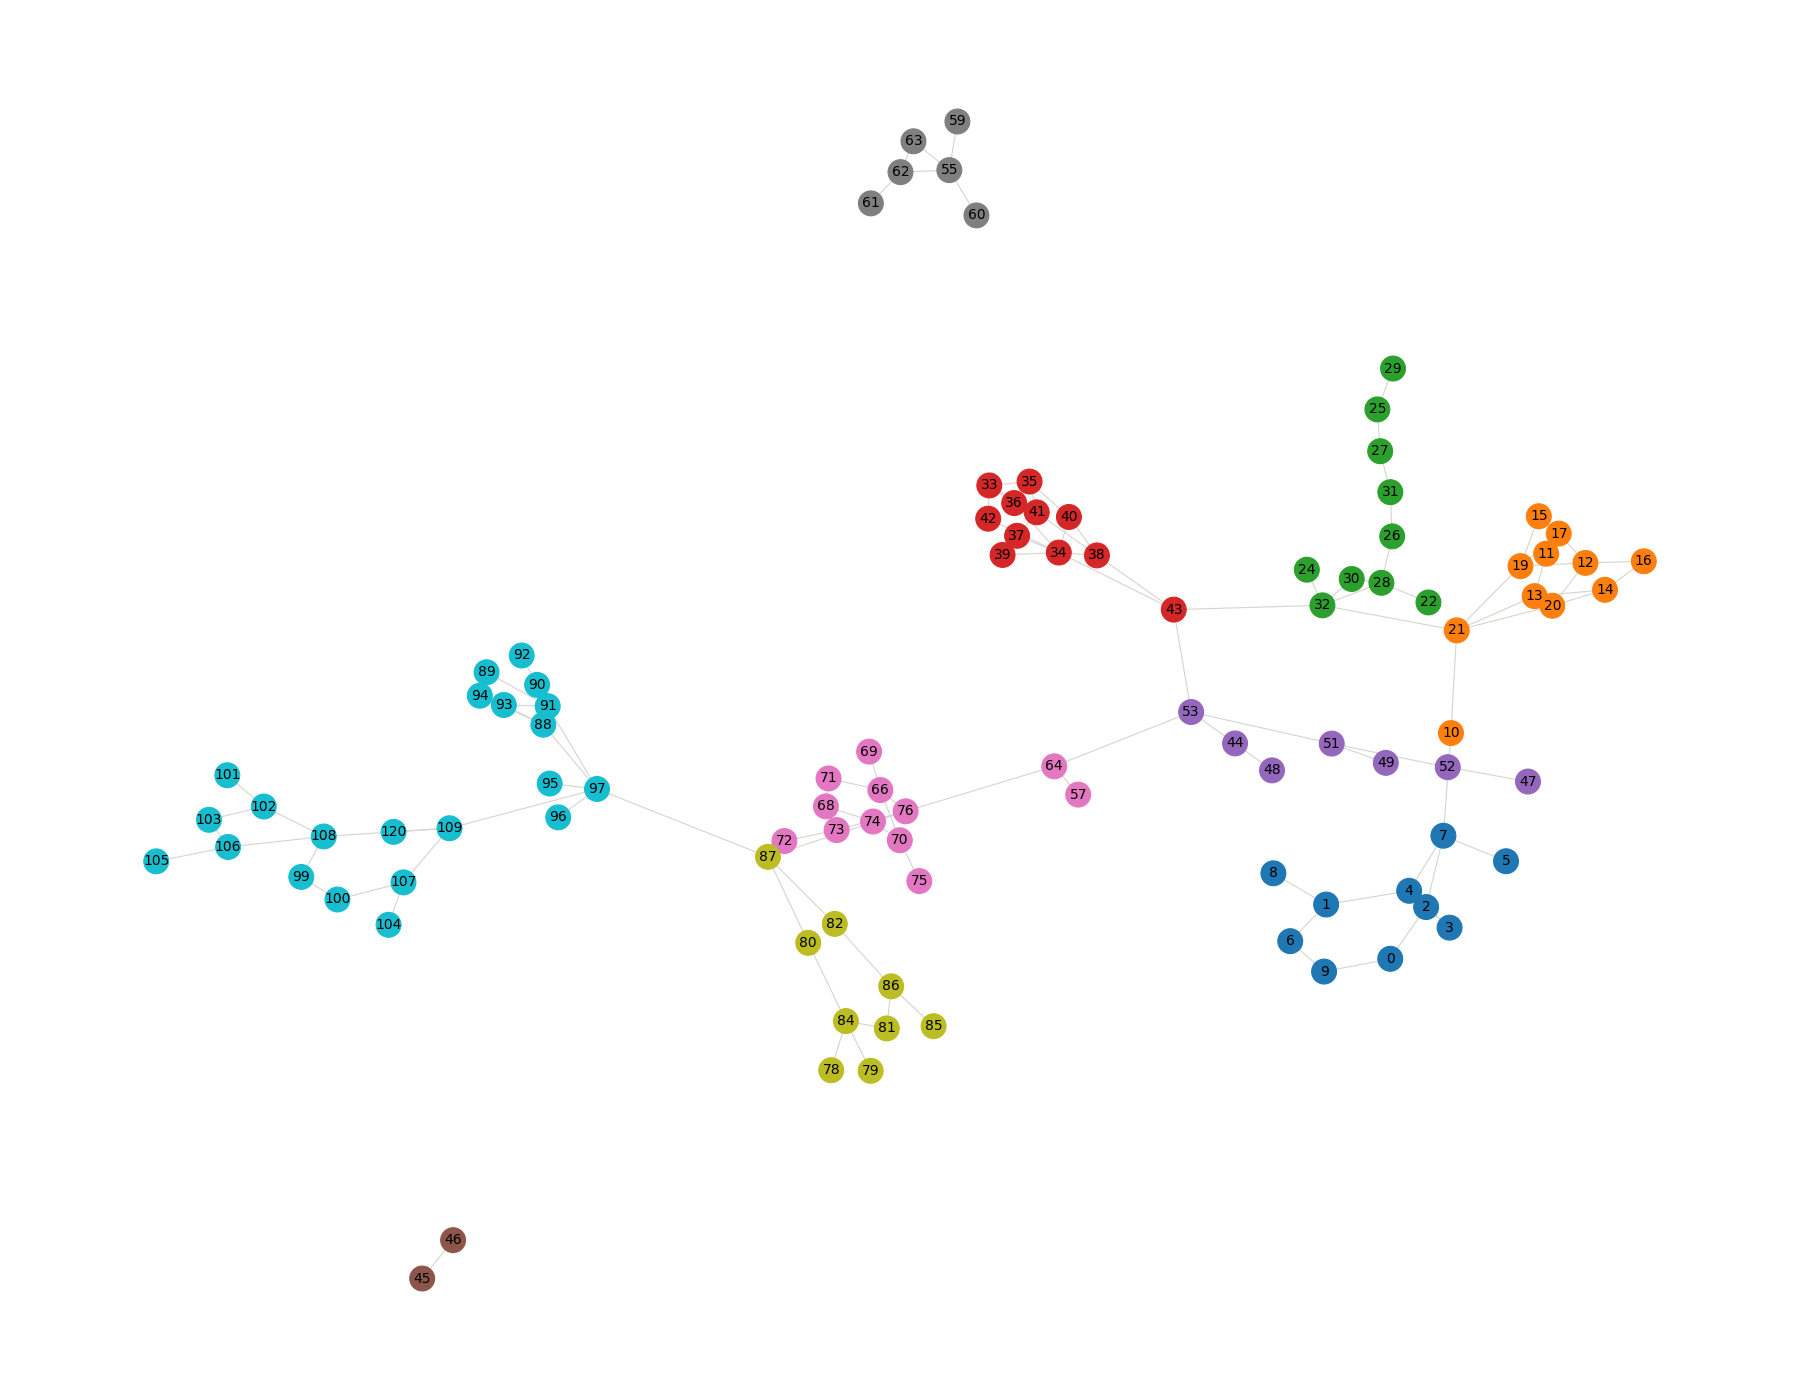
\includegraphics[width=1.0\textwidth]{Graphics/NearSocialNetwork.png}
    \caption{Random Soziale Graphen mit den höchsten Gradzentralitäts-Knoten als Verbindung }
    \label{NearSozialerGraph}
\end{figure}

\newpage
Nachdem der Plot \ref{NearSozialerGraph} durchaus \textit{Sozialen Netzwerken} ähnelt und die Werte der Berechnungen ebenfalls richtig erscheinen, müssen wir noch eine weitere Optimierung durchführen. Bei einer genaueren Betrachtung der Abbildung fällt auf, dass die Teilgraphen wenige Verbindungen untereinander aufweisen. Dies liegt an der Idee von \ref{uniteGraphs}, den Knoten mit der höchsten Gradzentralität zu wählen und diesen dann mit einer beliebigen weiteren Gruppe zu verbinden. Doch in tatsächlich ist ein solches Phänomen sehr unwahrscheinlich. Denn dies würde beispielsweise heißen, dass an der Universität Ulm alle Student(en)*innen der Fakultät für Ingenieurwissenschaften, Informatik und Psychologie untereinander in einer Weise miteinander verbunden sind, jedoch nur die Professor(en)*innen, welche die höchste Gradzentralität aufweisen, mit eine*m/r weiteren Professor*in einer anderen Fakultät verbunden sind. Dies ist aber nicht realistisch wenn bedacht wird, dass auch beispielsweise Student(en)*innen der Fakultät für Mathematik und Wirtschaftswissenschaften durchaus Kontakte zu der Fakultät für Ingenieurwissenschaften, Informatik und Psychologie haben können oder auch mit den jeweiligen Professor(en)*innen. Dementsprechend müssen wir diese Eigenschaft ebenfalls in der Implementierung berücksichtigen. Das kann gewährleistet werden, indem jedem Knoten eine zufällige Wahrscheinlichkeit zugeschrieben wird, die angibt, ob eine Kante zwischen den Subgraphen existiert. Hierzu ersetzen wir den Algorithmus \ref{uniteGraphs} ab Zeile \textit{17} zu:

\begin{algorithm}
\caption{Verbindung Subgraphen}\label{connection}
\begin{algorithmic}[1]
\Procedure{connection subgraphs}{}
\State $\textit{prob} \gets \text{zufällige Zahl, die sehr klein ist bis 0.00001}$
\For {\textit{i und j} liegen in der Matrix big graph}
\State \textit{befülle die Diagonale der Matrix mit 1}.
\EndFor
\For {\textit{i und k} liegen in der Matrix}
\State $\textit{variable} \gets \text{zufällige Zahl zwischen 0 und 1}$
\If{\textit{variable} kleiner \textit{prob}}
\State \textit{setze big graph [i][j] auf 1}
\EndIf
\EndFor
\EndFor
\textbf{RETURN} big graph
\EndProcedure
\end{algorithmic}
\end{algorithm}

Mit \ref{connection} können wir sicherstellen, dass die Subgraphen vermehrt miteinander verbunden sind und nicht von dem Knoten mit der höchsten Gradzentralität abhängen.

\section{Die Analyse des generierten Graphen}
Mit den Überlegungen aus 4.2 und den dort erklärten Methoden, lassen sich schließlich möglicherweise \textit{typische soziale Netzwerke} realisieren. Um zu beweisen, dass es sich tatsächlich um ein solches Netzwerk handelt, wollen wir ein neues generieren und eine Analyse darauf durchführen. Wir wollen zeigen, dass die mit dem Generator erzeugten Graphen tatsächlich näherungsweise \textit{sozialen Netzwerken} entsprechen.

\FloatBarrier
\begin{figure}[h!]
    \centering
    \hspace*{-2cm}
    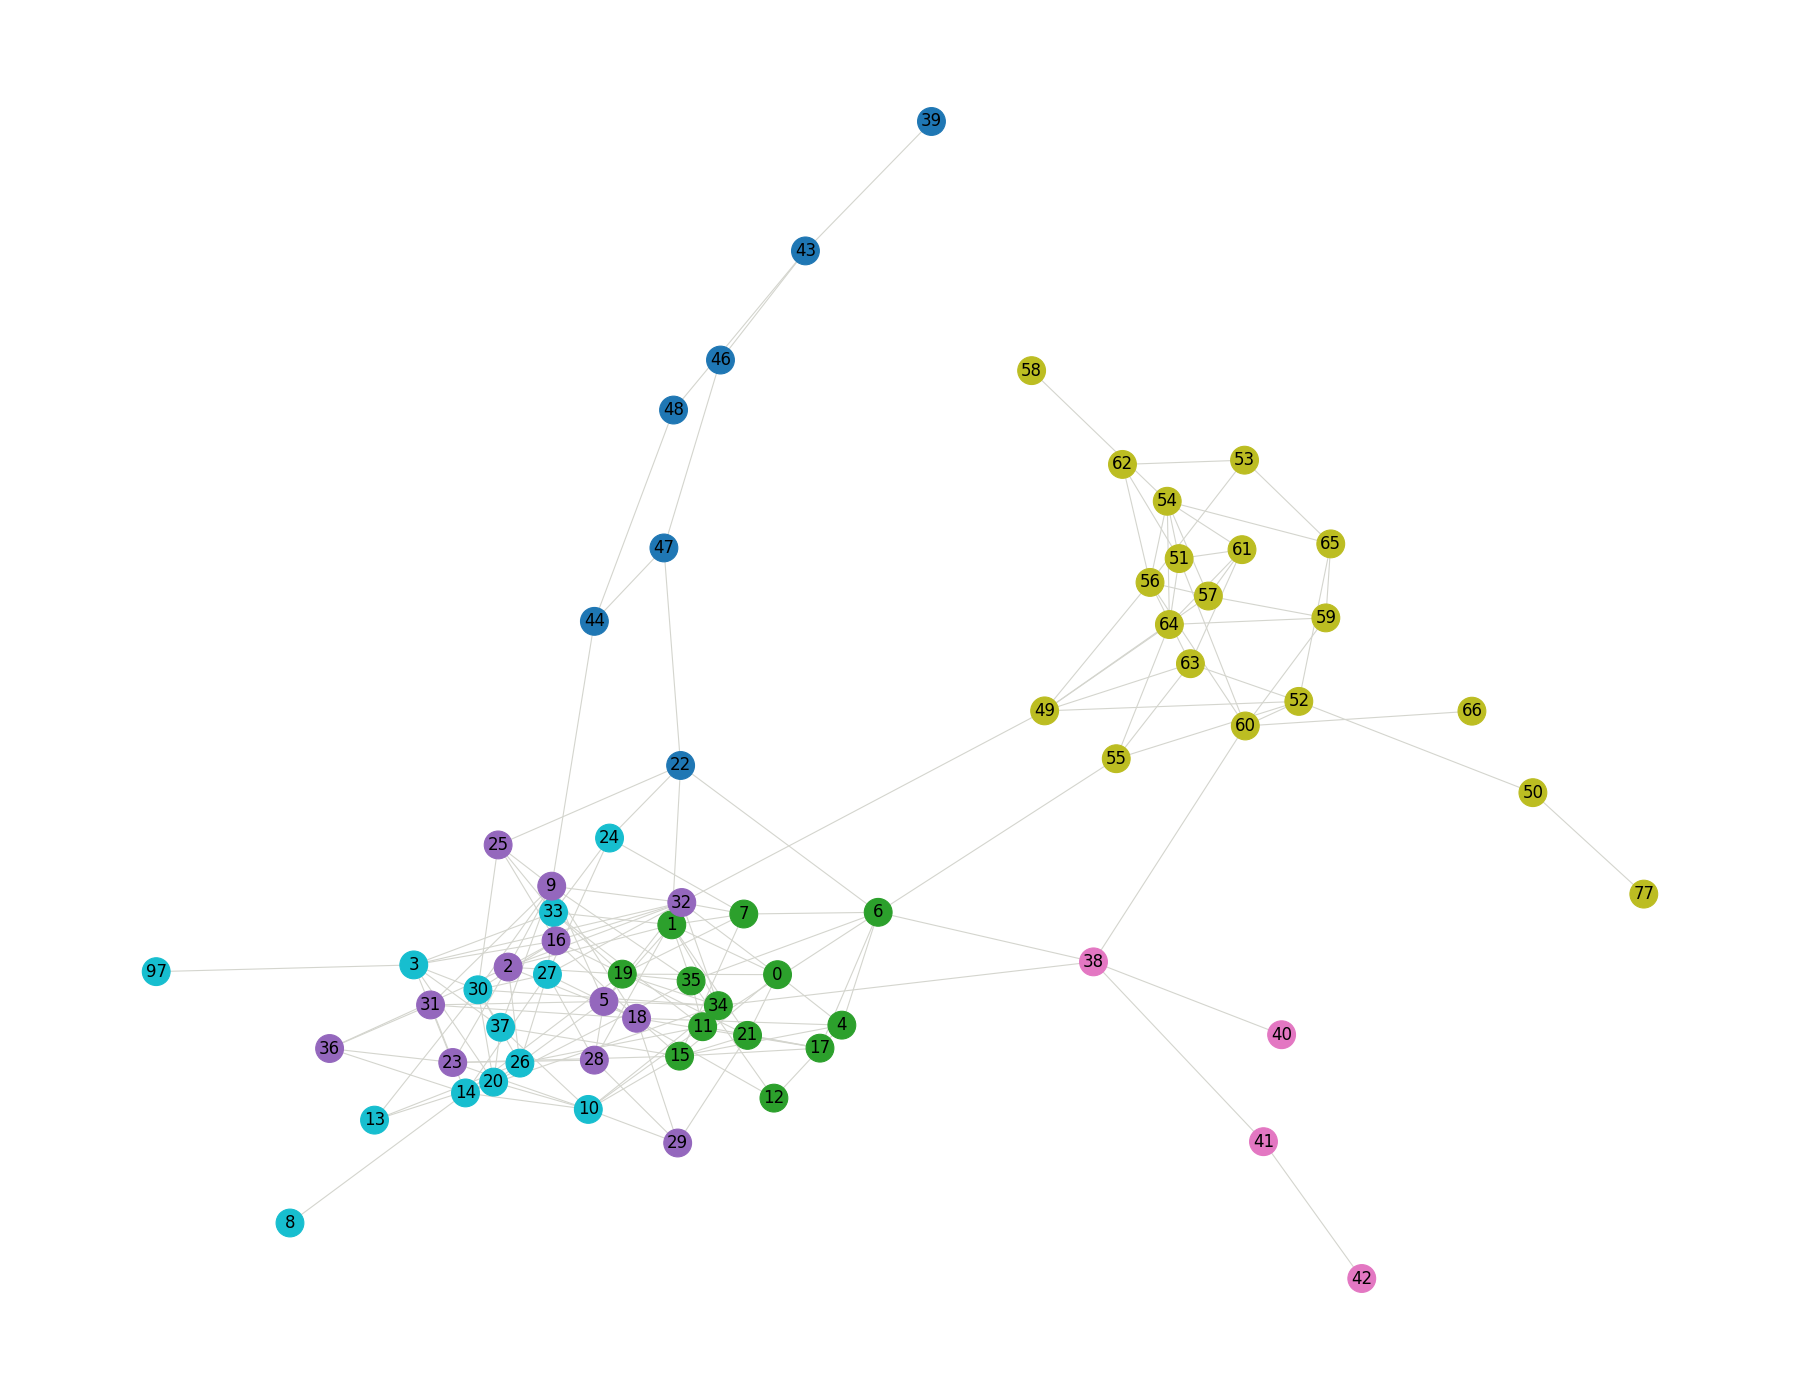
\includegraphics[width=0.8\textwidth]{Graphics/Random_moreConnections.png}
    \caption{Random soziales Netzwerk mit realistischeren Verbindungen}
    \label{fig:SNA}
\end{figure}

\FloatBarrier

Bei der visuellen Betrachtung des Plots \ref{fig:SNA} ähnelt die Struktur auf jeden Fall der, eines sozialen Netzwerks. Doch um eine fundierte Aussagen treffen zu können, wollen wir auch die Zentralitäten genauer analysieren. Hierfür wird folgende Tabelle verwendet:

\begin{table}[h!]
\footnotesize
\caption{Werte oberer Graph}
\begin{tabular}{lcccc}\toprule 
\textbf{Knoten} &\textbf{Grad-Zentr.} &\textbf{Nähe-Zentr.}  &\textbf{Between-Zentr.} \\
 &\\\midrule
  1 & 0.149254  & 0.389535 & 0.0429244   \\
  2 & 0.134328  & 0.370166 & 0.0366434   \\
  3 & 0.119403  & 0.350785 & 0.0516569   \\
  5 & 0.119403  & 0.378531 & 0.0341306   \\
  6 & 0.119403  & 0.385057 & 0.145038    \\
  7 & 0.0895522 & 0.358289 & 0.0208983   \\
 10 & 0.119403  & 0.341837 & 0.0240985   \\
 11 & 0.104478  & 0.360215 & 0.0212421   \\
 14 & 0.119403  & 0.3350    & 0.0454434   \\
 18 & 0.134328  & 0.340102 & 0.0283754   \\
 22 & 0.0746269 & 0.348958 & 0.0740623   \\
 27 & 0.119403  & 0.360215 & 0.0342121   \\
 30 & 0.149254  & 0.348958 & 0.0412278   \\
 32 & 0.179104  & 0.435065 & 0.266448    \\
 34 & 0.134328  & 0.394118 & 0.112543    \\
 35 & 0.104478  & 0.362162 & 0.0290967   \\
       
  \\\bottomrule
 \end{tabular}
  &
\begin{tabular}{lccc}
\toprule 
\textbf{Knoten} &\textbf{Grad-Zentr.} &\textbf{Nähe-Zentr.}  &\textbf{Between-Zentr.}\\
   &\\\midrule
 38 & 0.0746269 & 0.36612  & 0.154688    \\
 41 & 0.0298507 & 0.271255 & 0.0298507   \\
 43 & 0.0447761 & 0.198813 & 0.030303    \\
 44 & 0.0447761 & 0.295154 & 0.0773717   \\
 46 & 0.0298507 & 0.219672 & 0.0205638   \\
 47 & 0.0447761 & 0.27459  & 0.0520902   \\
 48 & 0.0298507 & 0.232639 & 0.0373285   \\
 49 & 0.0895522 & 0.36413  & 0.221288    \\
 50 & 0.0298507 & 0.241877 & 0.0298507   \\
 52 & 0.0895522 & 0.314554 & 0.0885577   \\
 54 & 0.104478  & 0.254753 & 0.0327816   \\
 55 & 0.0597015 & 0.325243 & 0.0670173   \\
 56 & 0.104478  & 0.303167 & 0.0672381   \\
 57 & 0.0746269 & 0.290043 & 0.0213757   \\
 60 & 0.0895522 & 0.313084 & 0.0903114   \\
 64 & 0.0895522 & 0.304545 & 0.0530434   \\
      \\\bottomrule
\end{tabular}
\end{table}
\label{TablleSNA}

Bei dieser Tabelle handelt es sich um die \textbf{32} wichtigsten Knoten. Die Anzahl der Knoten in der Tabelle \ref{TablleSNA} ist rein zufällig gewählt und hat keine Bedeutung. Alle Knoten die eine geringere \textbf{"Betweenness-Centrality"} kleineren als \textbf{0.02} aufweisen, sind außen vor gelassen. Auch hier haben wir die Grenze rein zufällig gewählt. Bei diesem Grenzwert handelt es sich um einen guten Mittelwert. Wir wollen weder zu wenig, noch zu viele Knoten betrachten.
Bei der Grad-Zentralität aus der Tabelle \ref{TablleSNA} sehen wir, dass die meisten Knoten einen Wert höher als \textbf{0.1} aufweisen. Wir können einen Schritt weitergehen und stellen schnell fest, dass einige wenige Knoten eine Grad-Zentralität höher als \textbf{0.13} aufweisen. Genau genommen handelt es sich hier um die Knoten \textbf{1} mit einem Wert von \textbf{0.149254}, den Knoten \textbf{2} mit dem Wert \textbf{0.134328}, Knoten \textbf{18} mit dem Wert \textbf{0.134328}, dann Knoten \textbf{30} mit einer Zentralität von \textbf{0.149254}, zudem um den Knoten \textbf{32} mit dem höchsten Wert von \textbf{0.179104} und schließlich Knoten \textbf{34} mit einer Grad-Zentralität von \textbf{0.134328}. All diese aufgezählten Knoten sind zentral wichtig für den Graphen und befinden sich höchstwahrscheinlich im Zentrum des Graphen \ref{fig:SNA}. Betrachten wir nun die Abbildung visuell, kann diese Behauptung teilweise bestätigt werden, denn die Knoten fallen direkt auf. Hohe Zentralitätswerte bei einem Knoten sagen aus, dass es sich beispielsweise im realen Leben um eine vermutlich sehr berühmte / bekannte Person handeln wird. Wir könnten annehmen, dass es ein Star, ein Influenzer oder eine, auf weitere Arten bekannte Person ist. Doch ebenso können wir annehmen, dass die Person lediglich viele andere Personen kennt, oder von vielen anderen Personen gekannt wird. Doch nicht nur die Grad-Zentralität spielt für uns und die Analyse in dieser Arbeit eine zentrale Rolle. Im Weiteren betrachten wir die \textbf{"Nähe-Zentralität"} doch um auch bei diesem Aspekt nicht alle \textbf{32} Werte aufzuzählen, betrachten wir im Folgenden nun Knoten, die einen Wert höher als \textbf{0.37} aufzeigen. Hierzu zählen der Knoten \textbf{1} mit einem Wert von \textbf{0.389535}, Konten \textbf{2} mit dem Wert \textbf{0.370166}, zudem Knoten \textbf{5} mit dem Wert \textbf{0.378531}, zusätzlich Knoten \textbf{6} mit der Zentralität \textbf{0.385057}, und schließlich die Knoten \textbf{32} mit dem höchsten Wert \textbf{0.435065} und \textbf{34} mit der Zentralität von \textbf{0.394118}. Je höher die Werte sind, so haben wir in dem ersten Teil der Arbeit gesehen, desto näher Befinden sich diese Knoten zu weiteren bzw. weisen die durchschnittlich kürzesten Wege auf. Betrachten wir nach dieser Information unseren Graphen \ref{fig:SNA} und suchen die Knoten mit der höchsten \textbf{Nähe-Zentralität}, sehen wir direkt, dass sich diese im gleichen Bereich befinden, wie die Knoten mit der höchsten \textbf{Grad-Zentralität}. Doch bestätigt der Plot unsere Vermutung nicht eindeutig, da es teilweise nicht ideal zu erkennen ist, ob die Kanten zum Knoten verlaufen oder an diesem vorbei, weshalb die ausschließlich visuelle Betrachtung eines Graphen oftmals nicht ausreichend ist. Zudem besteht auch die Möglichkeit, dass wir die Formeln nicht korrekt implementiert haben. Wobei händisches Nachrechnen, bei durchaus kleineren Plots, die Korrektheit dieser bewiesen hat, weshalb wir diese Vermutung in Klammern setzen und es daher tatsächlich an der nicht eindeutigen visuellen Darstellung liegen wird. Kommen wir zur letzten zu untersuchenden Zentralität, nämlich der \textbf{Betweenness-Zentralität}. Auch hier betrachten wir wieder die Knoten mit den höchsten Werten, und um nicht alle \textbf{32} Werte aufzuzählen, betrachten wir erneut nur Knoten mit einem Wert höher als \textbf{0.09}. Diese Voraussetzung erfüllen neben dem Knoten \textbf{6} mit dem Wert \textbf{0.145038} die Knoten \textbf{32} mit der höchsten Zentralität von \textbf{0.266448} und \textbf{34} mit einem Wert von \textbf{0.112543}, außerdem der Knoten \textbf{38} mit der Zentralität von \textbf{0.154688}, zudem der Knoten \textbf{49} mit dem Wert \textbf{0.221288} und schließlich der Knoten \textbf{60} mit dem Wert \textbf{0.0903114}. Das bedeutet für unseren Graphen \ref{fig:SNA}, dass die kürzesten Wege anteilsmäßig am öftesten über diese genannten Knoten verlaufen. Betrachten wir erneut den Graphen, sehen wir eine zum Teil bekannte Eigenschaft, dass sich die Punkte im grün, lila, hellblau verschmolzenen, links unten zentrierten, drei Teilgraphen befinden. Doch kommt bei der \textbf{Betweenness-Zentralität} hinzu, dass sich die Knoten \textbf{49 und 60} auch im gelbgrünen, rechts oben liegenden, Teilgraphen befinden. In diesem Fall sehen wir eindeutig, dass die Werte gut zu unserem Plot passen und es sehr wahrscheinlich ist, dass unsere Annahme korrekt ist, und die Knoten tatsächlich am häufigsten bei allen kürzesten Wegen durchlaufen werden. Weitere Zentralitätswerte werden wir nicht betrachten. Nachdem wir alle Kriterien überprüft und erfolgreich festgestellt, dass dieser Graph einem \textbf{sozialen Netzwerk} ähnelt, möchten wir untersuchen, dass wir nicht zufällig einen passenden Graphen erhalten haben. Deshalb möchten wir uns noch ein weiteres Kriterium für die Zentralitäten überlegen und anschließend untersuchen.


\section{Die Verteilung der Zentralitäten}
Nachdem wir im vorherigen Kapitel die Generierung eines \textbf{sozialen Netzwerkes} und die Analyse durchgeführt haben, möchten wir uns im Folgenden die Verteilung der Zentralitätswerte anschauen.
Im Laufe der Arbeit ist aufgefallen, dass sich die Werte der Zenralitäten oftmals in ähnlichen Zahlenbereichen befinden. An dieser Stelle können wir uns die Frage stellen, wie diese Werte verteilt sind und ob die Verteilung einer mathematischen Wahrscheinlichkeitsverteilung entspricht. Das heißt, im Konkreten, wollen wir der Frage nachgehen, ob alle Zentralitätswerte sozialer Netzwerke ähnliche Verteilungen nachweisen. Würde sich unsere Vermutung diesbezüglich bestätigen, können wir andere soziale Netzwerke anhand dieses Kriterium vergleichen.
Da der Graph \ref{fig:SNA} ein zufällig, einmalig erzeugter Graph ist, werden wir einen neuen Graphen in unserem Generator erzeugen, um die Verteilung der Zentralitäten zu betrachten. Dies wird sich nicht auf die Untersuchung auswirken, denn die Verteilungen der Zentralitäten unserer Graphen sollte grob gleich oder zumindest ähnlich sein. Bei der erneuten Generierung erhalten wir nun folgenden Graphen und die zugehörige Verteilung der \textbf{Gradzentralität}:

\FloatBarrier
\begin{figure}[h!]%
  \centering
  \subfloat[][]{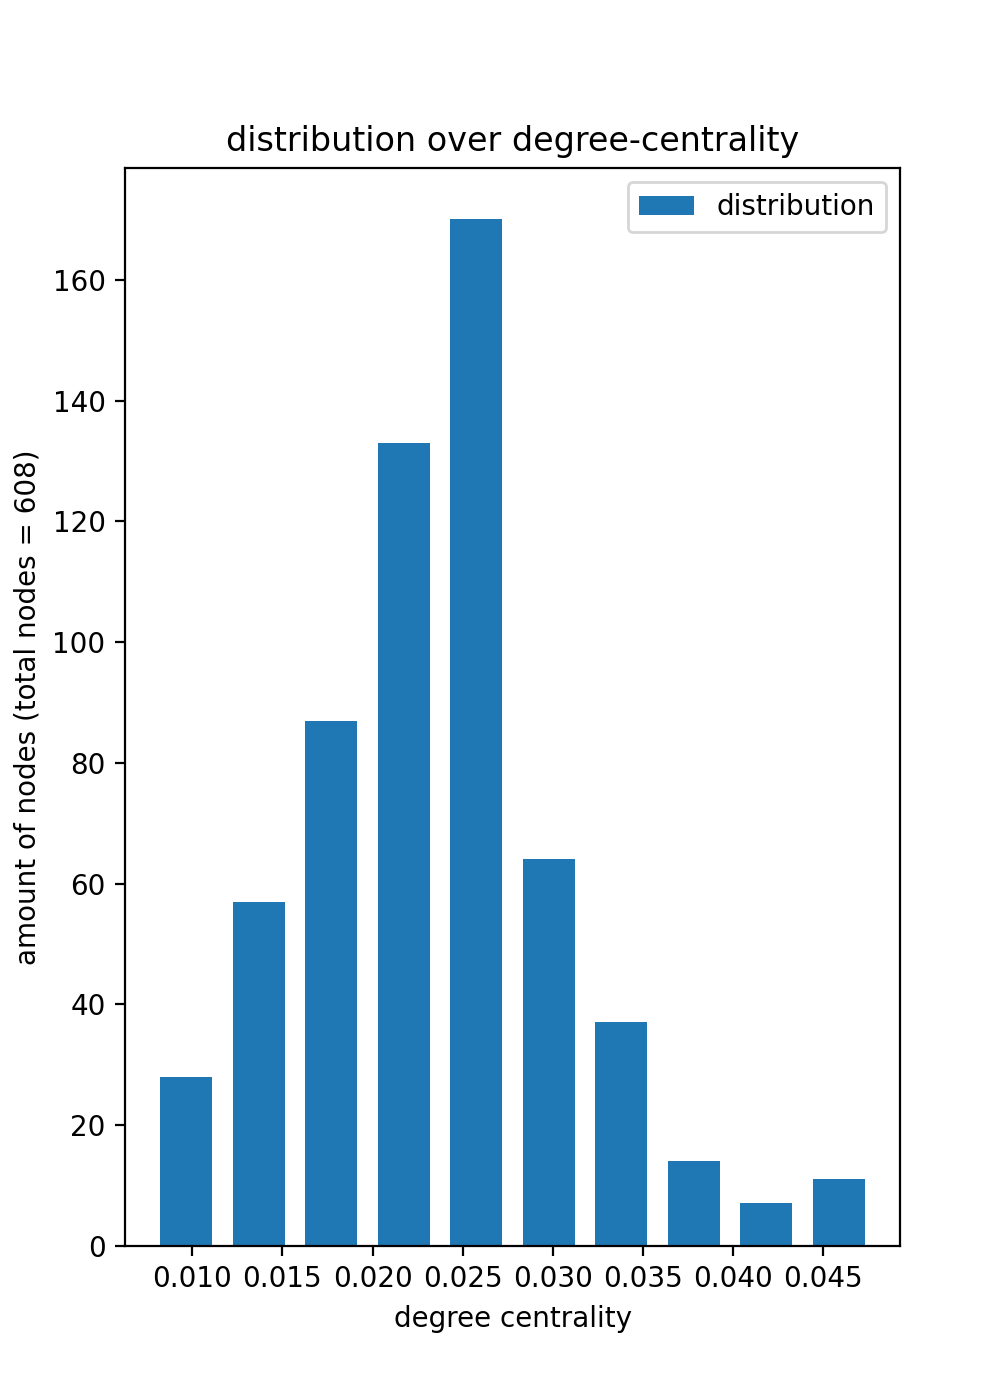
\includegraphics[width=0.4\linewidth]{Graphics/distribution_degree.png}}%
  \qquad
  \subfloat[][]{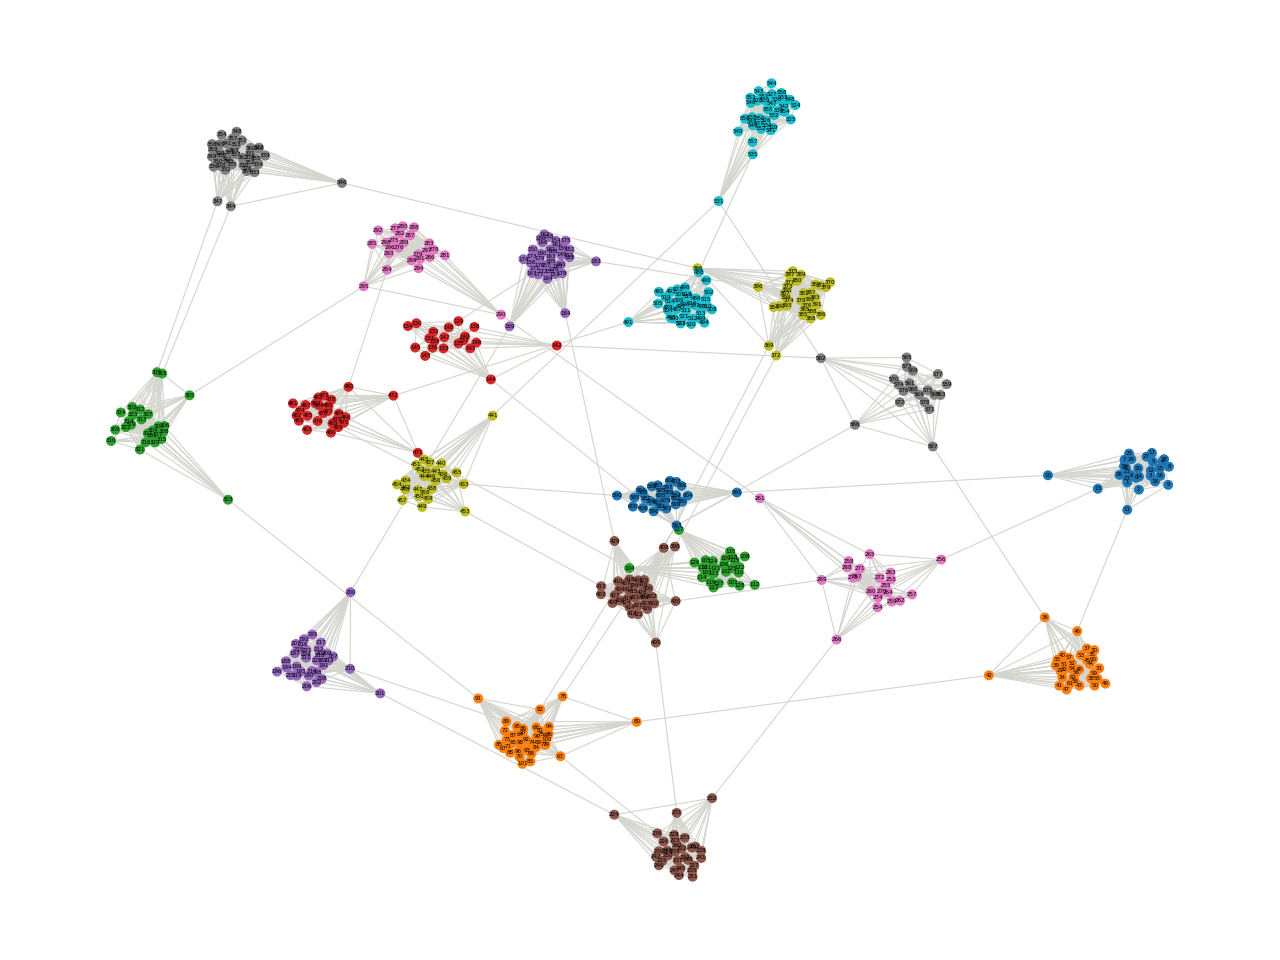
\includegraphics[width=0.5\linewidth]{Graphics/plot_degreeDist.png}}%
  \caption{Verteilung der Grad-Zentralität des Graphen (b)}%
  \label{fig:distribution}
\end{figure}
\FloatBarrier

Wir sehen, dass die \textbf{Gradzentralität} normal- beziehunsgweise gaußverteilt ist. Natürlich ist zu erwähnen, dass wir keine perfekte Gauß-Verteilung sehen, sondern eine etwas nach links verschobene Verteilung. Was die möglichen Gründe dafür sind, werden wir uns später anschauen und versuchen zu korrigieren. Nun wollen wir untersuchen, ob sich die Eigenschaft, der  normalverteilten Zentralitäten für die \textbf{Nähe-} und \textbf{Betweenness-Zentralität} ebenfalls bestätigen lässt. Um zusätzlich zu beweisen, dass es sich bei der Gauß-Verteilung der Werte nicht um einen Zufall handelt, generieren wir einen neuen sozialem Graphen und untersuchen die Verteilung der \textbf{Grad-}, \textbf{Nähe-}, \textbf{Betweenness-} und \textbf{Eigenvektor-Zentralität}. Hierbei stellen wir uns vor allem die Frage, ob die Verteilung einer tatsächlichen Normalverteilung entspricht und falls ja, warum dies der Fall ist. Ansonsten stellen wir uns die Frage warum es keiner Normalverteilung entspricht und ob es möglich ist, den Graphen zu verändern um eine solche zu erzielen. Bei der erneuten Generierung erhalten wir schließlich folgenden Graphen:

\FloatBarrier
\begin{figure}[h!]%
  \centering
  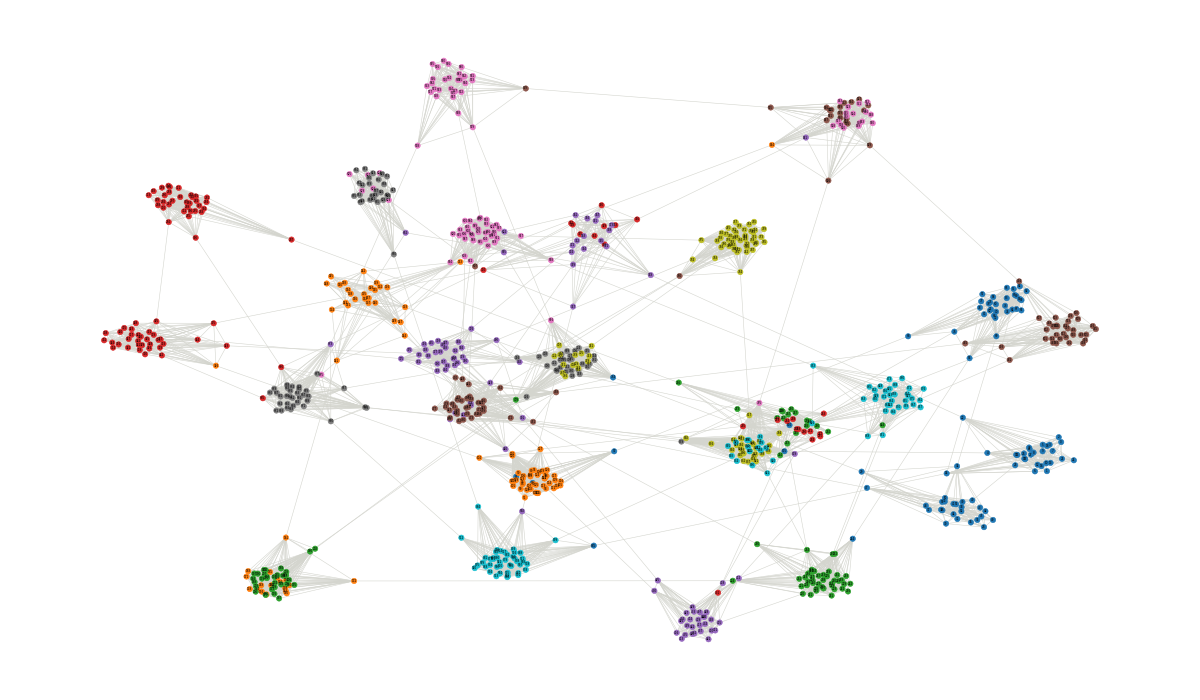
\includegraphics[width=0.8\textwidth]{Graphics/newourSN.png}
  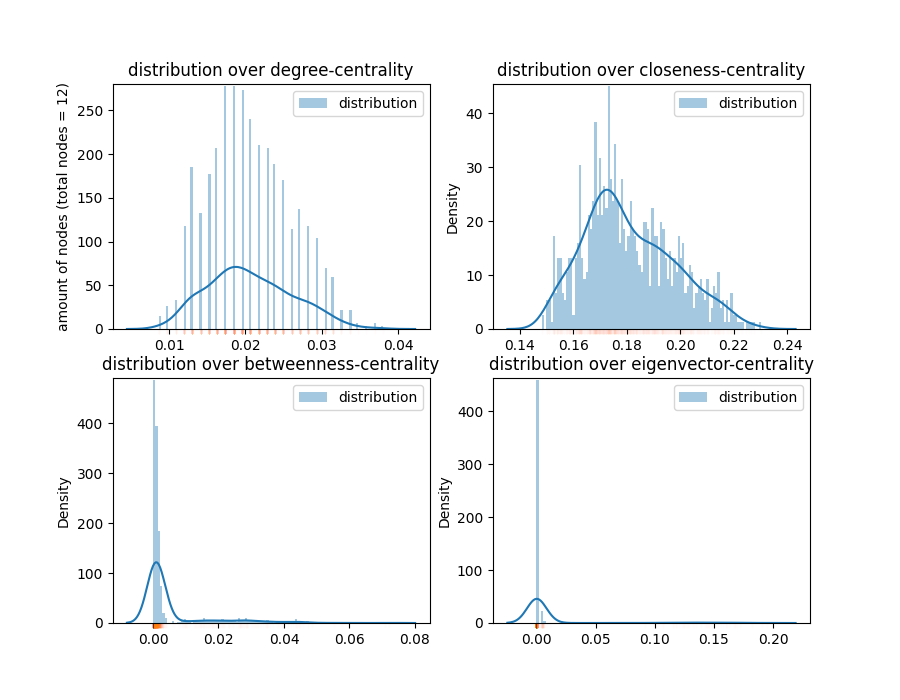
\includegraphics[width=1.0\textwidth]{Graphics/newOurDist.png}
  \caption{Random soziales Netzwerk mit realistischeren Verbindungen}
  \label{fig:distributionALL}
\end{figure}
\FloatBarrier
In der Abbildung \ref{fig:distributionALL} sehen wir nun die Verteilungen der Zentralitäten von dem, sich darunter befindenden, sozialen Netzwerks. Die Tabelle mit den Zentralitäts-Werten des Netzwerks befindet sich als Datei in \cite{TZ}. Oben links sehen wir die Verteilung der \textbf{Grad-Zentralität}, welche wie bereits oben festgestellt, nicht exakt normalverteilt ist, aber Ähnlichkeiten zu erkennen sind. Vor allem auffällig ist, dass der Balken bei \textbf{0.012} vergleichsweise sehr hoch ist. Über \textbf{50} Knoten weisen diesen Wert auf. Danach geht der darauf folgende Balken nochmals zurück, denn nur noch etwas über \textbf{25} Knoten haben eine Zentralität von circa \textbf{0.03}. Wir haben jedoch erwartet, dass sich das Balkendiagramm typischerweise symmetrisch verhält, doch das Gegenteil tritt ein. Über \textbf{150} Knoten weisen eine Zentralität von \textbf{0.0125} auf, daher sollten auch ebenso viele den Wert \textbf{0.025} besitzen. Hingegen ist positiv hervorzuheben, dass wir genau \textbf{einen Peak} erreichen, wie wir auch erwartet haben. Außerdem sind alle Balken vor dem Peak kontinuierlich aufsteigend und nach dem Peak kontinuierlich absteigend. Doch lediglich eine Unstimmigkeit sticht hier heraus, bei dem Zentralitätswert von \textbf{0.0357} den etwas unter \textbf{25} Knoten besitzen. Fraglich ist hier, warum der Balken erneut höher ist als sein Vorgänger. Denn im Regelfall sollten wir maximal ein bis drei Knoten finden, die diesen Wert aufweisen. Doch im Allgemeinen weist der Plot genau die Eigenschaft nach, die wir auch erwartete haben, nämlich dass die \textbf{Grad-Zentralität} annähernd normalverteilt ist. Wenn wir nun zu dem Balkendiagramm der \textbf{Nähe-Zentralität bzw. closeness-centrality} blicken, sehen wir einen ähnlichen Verlauf. Wir entdecken einen bereits erwarteten Peak und weitere Balken, die im linken Bereich sehr schnell zum Peak hin ansteigen und rechts vom Peak vergleichsweise langsam abflachen. Sehr analog zu dem Balkendiagramm der \textbf{Grad-Zentralität}. Auffällig ist erneut, dass der letzte Balken wider Erwartens höher ist als der Balken davor. Die Vermutung liegt nahe, dass es sich hier um einen Zufall handelt. Wir haben viele Generierungen durchgeführt und in \ref{ch:anhang} befinden sich ebenso weitere Balkendiagramme und Soziale Netzwerke. Aussagen die wir auf jeden Fall sicher treffen können ist, dass falls es zu Unstimmigkeiten kommt diese stets an anderen Stellen auftreten und nicht immer den letzten Balken betreffen. Diese Aussage können wir jedoch nur für die Verteilung der \textbf{Grad-} und \textbf{Nähe-Zentralitäten} treffen. Jedoch könne wir ebenso annhehmen, dass je größer der Graph ist, umso eher sind diese Zentralitäten normalverteilt. Was daran liegt, dass wir mehr Knoten haben und diese irgendwann eine Regelmäßigkeit aufzeigen. Grob angedeutet, kann die Existenz einer Kante als Binomialverteilung interpretiert werden und diese konvergiert mathematisch gesehen bei einer sehr großen Stichprobe (Anzahl an Knoten in unserem Fall) gegen eine Normal- bzw Gaußverteilung.
Doch schauen wir uns auch noch die zwei unteren Balkendiagramme an, wird unsere Behauptung verworfen. Bei der \textbf{Betweenness-} und \textbf{Eigenvektor-Zentralität} wird unsere angenommene Regelmäßigkeit nicht bestätigt. Zum einen weisen die Balken wenige unterschiedliche Werte auf, die teilweise kaum zu unterscheiden sind. Was zudem auffällt, sind die Ausschläge der vorderen Balken. Was zunächst verwunderlich erscheint, ist mit einer simplen Erklärung begründet. Die \textbf{Closeness-Zentralität} gibt bekanntlich an, wie oft ein Knoten anteilsmäßig bei der Suche nach dem kürzesten Weg durch einen Graphen benutzt wird. Der Ausschlag ist daher die Folge davon, wenn viele kürzeste Wege stets über die gleichen Knoten verlaufen. Das heißt, es existieren keine bis wenige Alternativen und so verlaufen die kürzesten Wege von beispielsweise \textbf{Knoten 1} zu einem weiteren Knoten stets über gleiche beziehungsweise ähnliche Knoten. Bei der \textbf{Eigenvektor-Zentralität} haben wir zwar die gleiche Beobachtung gemacht doch sagt diese hier etwas anderes aus. Diese Zentralität gibt uns eine Einschätzung der Wichtigkeit des Knotens, im Bezug auf seine Nachbarn an, was bezogen auf unser Balkendiagramm heißt, dass viele Knoten in unserem Graphen wichtig sind mit Einbeziehung der Nachbarn. Wobei wir auch vermuten können, dass dies mit der hohen Anzahl an Konten mit höher \textbf{Betweenness-Zentralität} zusammenhängt. 
Die komplette Analyse des sozialen Netzwerks in \ref{fig:distributionALL} befindet sich in \cite{TZ}, da wir uns bereits eine ausführliche Analyse durchgeführt haben. Danach zu Urteilen handelt es sich bei dem Netzwerk um ein typisches \textbf{soziales Netzwerk}.

\section{Kurzes Recap}
Nachdem wir uns nun angeschaut haben, wie wir soziale Netzwerke generieren können, sehen wir auch gleichzeitig die Probleme dieser. Zudem haben wir unseren Code fortlaufend optimiert und ein soziales Netzwerk erstellt. Für dieses haben wir danach eine soziale Netzwerk Analyse erstellt und festgestellt, dass es die Anforderungen an ein soziales Netzwerk erfüllt werden. Danach ist uns aufgefallen, dass die Zentralitäten regelmäßig sind und konnten die Normalverteilung nachweisen. Doch müssen wir uns im Folgenden die Frage stellen, wie die Verteilung der Zentralitäten bei anderen, bereits analysierten Netzwerken aussieht.
